\section{Greenplum Database}
\label{sec:greenplum}

\href{http://greenplum.org/}{Greenplum Database (GP)}~--- реляционная СУБД, имеющая массово-параллельную (massive parallel processing) архитектуру без разделения ресурсов (shared nothing). Для подробного понимания принципов работы Greenplum необходимо обозначить основные термины:

\begin{itemize}
  \item Master instance (<<мастер>>)~--- инстанс PostgreSQL, являющийся одновременно координатором и входной точкой для пользователей в кластере;
  \item Master host (<<сервер-мастер>>)~--- сервер, на котором работает master instance;
  \item Secondary master instance~--- инстанс PostgreSQL, являющийся резервным мастером, включается в работу в случае недоступности основного мастера (переключение происходит вручную);
  \item Primary segment instance (<<сегмент>>)~--- инстанс PostgreSQL, являющийся одним из сегментов. Именно сегменты непосредственно хранят данные, выполняют с ними операции и отдают результаты мастеру (в общем случае). По сути сегмент~--- самый обычный инстанс PostgreSQL 8.3.23 с настроенной репликацией в своё зеркало на другом сервере;
  \item Mirror segment instance (<<зеркало>>)~--- инстанс PostgreSQL, являющийся зеркалом одного из primary сегментов, автоматически принимает на себя роль primary в случае падения оного. Greenplum поддерживает только 1-to-1 репликацию сегментов: для каждого из primary может быть только одно зеркало;
  \item Segment host (<<сервер-сегмент>>)~--- сервер, на котором работает один или несколько сегментов и/или зеркал;
\end{itemize}

В общем случае кластер GP состоит из нескольких серверов-сегментов, одного сервера-мастера, и одного сервера-секондари-мастера, соединённых между собой одной или несколькими быстрыми (10g, infiniband) сетями, обычно обособленными (interconnect) (рис~\ref{fig:greenplum_arch1}).

\begin{figure}[h!]
  \center{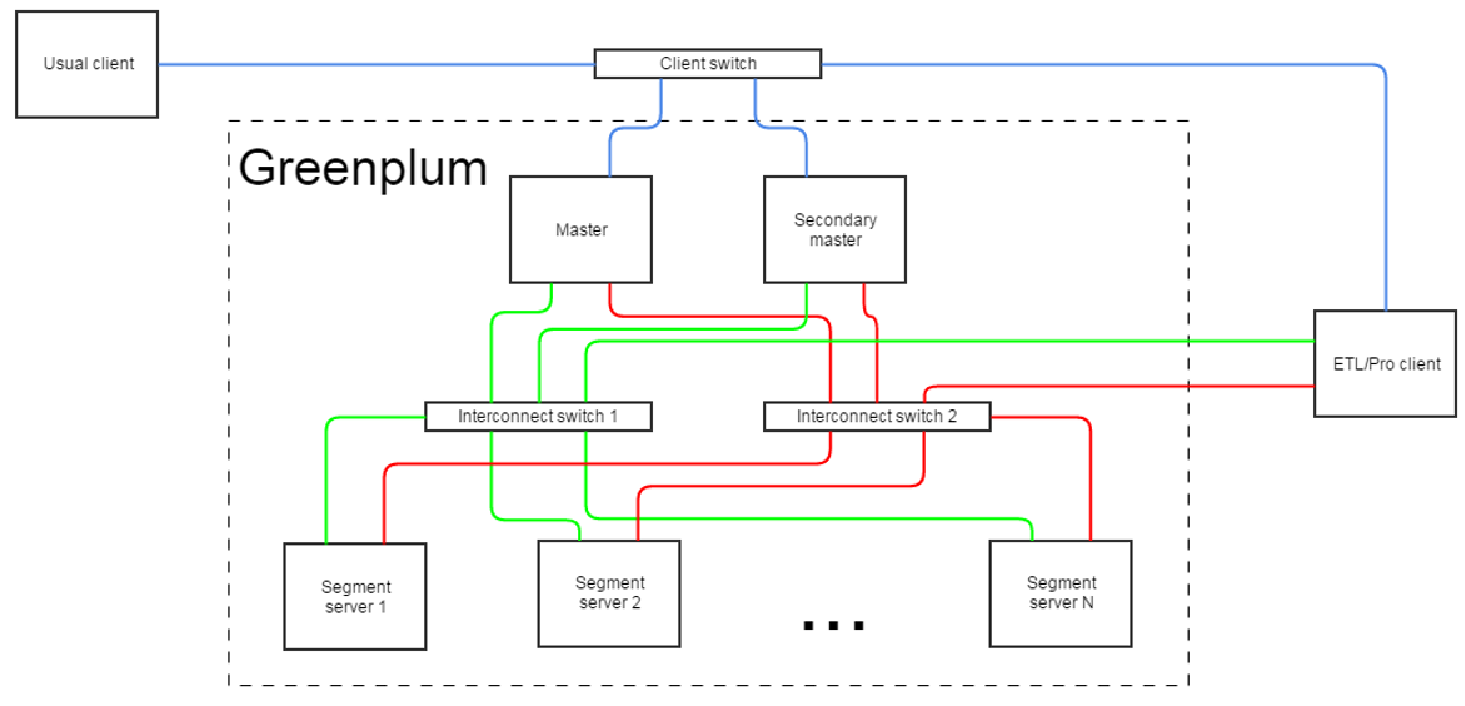
\includegraphics[width=1\textwidth]{greenplum-basic-arch.pdf}}
  \caption{Состав кластера и сетевое взаимодействие элементов. Зелёная и красная линии~--- обособленные сети interconnect, синяя линия~--- внешняя, клиентская сеть}
  \label{fig:greenplum_arch1}
\end{figure}

Использование нескольких interconnect-сетей позволяет, во-первых, повысить пропускную способность канала взаимодействия сегментов между собой, и во-вторых, обеспечить отказоустойчивость кластера (в случае отказа одной из сетей весь трафик перераспределяется между оставшимися).

При выборе числа серверов-сегментов важно правильно выбрать соотношение кластера <<число процессоров/Тб данных>> в зависимости от планируемого профиля нагрузки на БД~--- чем больше процессорных ядер приходится на единицу данных, тем быстрее кластер будет выполнять <<тяжёлые>> операции, а также работать со сжатыми таблицами.

При выборе числа сегментов в кластере (которое в общем случае к числу серверов никак не привязано) необходимо помнить следующее:

\begin{itemize}
  \item все ресурсы сервера делятся между всеми сегментами на сервере (нагрузкой зеркал, в случае если они располагаются на этих же серверах, можно условно пренебречь);
  \item каждый запрос на одном сегменте не может потреблять процессорных ресурсов больше, чем одно ядро CPU. Это означает, например, что, если кластер состоит из 32-ядерных серверов с 4-я сегментами GP на борту и используется в среднем для обработки 3-4 одновременных тяжёлых, хорошо утилизирующих CPU, запросов, <<в среднем по больнице>> CPU не будет утилизироваться оптимально. В данной ситуации лучше увеличить число сегментов на сервере до 6-8;
  \item штатный процесс бекапа и рестора данных <<из коробки>> работает только на кластерах, имеющих одинаковое число сегментов. Восстановить данные, забекапленные на кластере из 96 сегментов, в кластер из 100 сегментов без напильника будет невозможно;
\end{itemize}


\subsection{Хранение данных}
\label{subsec:greenplum_data_storage}

В Greenplum реализуется классическая схема шардирования данных. Каждая таблица представляет из себя N+1 таблиц на всех сегментах кластера, где N~--- число сегментов (+1 в этом случае — это таблица на мастере, данных в ней нет). На каждом сегменте хранится 1/N строк таблицы. Логика разбиения таблицы на сегменты задаётся ключом (полем) дистрибуции~--- таким полем, на основе данных которого любую строку можно отнести к одному из сегментов.

Ключ (поле или набор полей) дистрибуции~--- очень важное понятие в GP. Как было сказано выше, Greenplum работает со скоростью самого медленного сегмента, это означает, что любой перекос в количестве данных (как в рамках одной таблицы, так и в рамках всей базы) между сегментами ведёт к деградации производительности кластера, а также к другим проблемам. Именно поэтому следует тщательно выбирать поле для дистрибуции~--- распределение количества вхождений значений в нём должно быть как можно более равномерным. Правильно ли вы выбрали ключ дистрибуции вам подскажет служебное поле \lstinline!gp_segment_id!, существующее в каждой таблице~--- оно содержит номер сегмента, на котором хранится конкретная строка. Важный нюанс: GP не поддерживает \lstinline!UPDATE! поля, по которому распределена таблица.

Рассмотрим пример (здесь и далее в примерах кластер состоит из 96 сегментов):

\begin{lstlisting}[language=SQL,label=lst:greenplum_example1,caption=Создание распределенной таблицы]
db=# create table distrib_test_table as select generate_series(1,20) as num_field distributed by (num_field);
SELECT 20
db=# select count(1),gp_segment_id from distrib_test_table group by gp_segment_id order by gp_segment_id;
 count | gp_segment_id
-------+---------------
     1 |             4
     1 |             6
     1 |            15
     1 |            21
     1 |            23
     1 |            25
     1 |            31
     1 |            40
     1 |            42
     1 |            48
     1 |            50
     1 |            52
     1 |            65
     1 |            67
     1 |            73
     1 |            75
     1 |            77
     1 |            90
     1 |            92
     1 |            94

db=# truncate table distrib_test_table;
TRUNCATE TABLE
db=# insert into distrib_test_table values (1), (1), (1), (1), (1), (1), (1), (1), (1), (1), (1), (1), (1), (1), (1), (1), (1), (1), (1), (1);
INSERT 0 20
db=# select count(1),gp_segment_id from distrib_test_table group by gp_segment_id order by gp_segment_id;
 count | gp_segment_id
-------+---------------
    20 |            42
\end{lstlisting}

В обоих случаях распределена таблица по полю \lstinline!num_field!. В первом случае вставили в это поле 20 уникальных значений, и, как видно, GP разложил все строки на разные сегменты. Во втором случае в поле было вставлено 20 одинаковых значений, и все строки были помещены на один сегмент.

В случае, если в таблице нет подходящих полей для использования в качестве ключа дистрибуции, можно воспользоваться случайной дистрибуцией (\lstinline!DISTRIBUTED RANDOMLY!). Поле для дистрибуции можно менять в уже созданной таблице, однако после этого её необходимо перераспределить.
Именно по полю дистрибуции Greenplum совершает самые оптимальные \lstinline!JOIN!: в случае, если в обоих таблицах поля, по которым совершается \lstinline!JOIN!, являются ключами дистрибуции, \lstinline!JOIN! выполняется локально на сегменте. Если же это условие не верно, GP придётся или перераспределить обе таблицы по искомому полю, или закинуть одну из таблиц целиком на каждый сегмент (операция \lstinline!BROADCAST!) и уже затем джойнить таблицы локально на сегментах.

\begin{lstlisting}[language=SQL,label=lst:greenplum_example2,caption=JOIN по ключу дистрибуции]
db=# create table distrib_test_table as select generate_series(1,192) as num_field, generate_series(1,192) as num_field_2 distributed by (num_field);
SELECT 192
db=# create table distrib_test_table_2 as select generate_series(1,1000) as num_field, generate_series(1,1000) as num_field_2 distributed by (num_field);
SELECT 1000
db=# explain select * from distrib_test_table sq
db-# left join distrib_test_table_2 sq2
db-# on sq.num_field = sq2.num_field;
QUERY PLAN
------------------------------------------------------------------------------------------
 Gather Motion 96:1  (slice1; segments: 96)  (cost=20.37..42.90 rows=861 width=16)
   ->  Hash Left Join  (cost=20.37..42.90 rows=9 width=16)
         Hash Cond: sq.num_field = sq2.num_field
         ->  Seq Scan on distrib_test_table sq  (cost=0.00..9.61 rows=9 width=8)
         ->  Hash  (cost=9.61..9.61 rows=9 width=8)
               ->  Seq Scan on distrib_test_table_2 sq2  (cost=0.00..9.61 rows=9 width=8)
\end{lstlisting}

\begin{lstlisting}[language=SQL,label=lst:greenplum_example3,caption=JOIN не по ключу дистрибуции]
db_dev=# explain select * from distrib_test_table sq left join distrib_test_table_2 sq2
on sq.num_field_2 = sq2.num_field_2;
                                               QUERY PLAN
--------------------------------------------------------------------------------------------------------
 Gather Motion 96:1  (slice3; segments: 96)  (cost=37.59..77.34 rows=861 width=16)
   ->  Hash Left Join  (cost=37.59..77.34 rows=9 width=16)
         Hash Cond: sq.num_field_2 = sq2.num_field_2
         ->  Redistribute Motion 96:96  (slice1; segments: 96)  (cost=0.00..26.83 rows=9 width=8)
               Hash Key: sq.num_field_2
               ->  Seq Scan on distrib_test_table sq  (cost=0.00..9.61 rows=9 width=8)
         ->  Hash  (cost=26.83..26.83 rows=9 width=8)
               ->  Redistribute Motion 96:96  (slice2; segments: 96)  (cost=0.00..26.83 rows=9 width=8)
                     Hash Key: sq2.num_field_2
                     ->  Seq Scan on distrib_test_table_2 sq2  (cost=0.00..9.61 rows=9 width=8)


\end{lstlisting}


Как видно в примере <<\nameref{lst:greenplum_example3}>> в плане запроса появляются два дополнительных шага (по одному для каждой из участвующих в запросе таблиц): \lstinline!Redistribute Motion!. По сути, перед выполнением запроса GP перераспределяет обе таблицы по сегментам, используя логику поля \lstinline!num_field_2!, а не изначального ключа дистрибуции~--- поля \lstinline!num_field!.


\subsection{Взаимодействие с клиентами}

В общем случае всё взаимодействие клиентов с кластером ведётся только через мастер~--- именно он отвечает клиентам, выдаёт им результат запроса и т.д. Обычные клиенты не имеют сетевого доступа к серверам-сегментам.

Для ускорения загрузки данных в кластер используется bulk load~--- параллельная загрузка данных с/на клиент одновременно с нескольких сегментов. Bulk load возможен только с клиентов, имеющих доступ в интерконнекты. Обычно в роли таких клиентов выступают ETL-сервера и другие системы, которым необходима загрузка большого объёма данных (на рис~\ref{fig:greenplum_arch1} они обозначены как ETL/Pro client).

Для параллельной загрузки данных на сегменты используется утилита \lstinline!gpfdist!. По сути, утилита поднимает на удалённом сервере web-сервер, который предоставляет доступ по протоколам gpfdist и http к указанной папке. После запуска директория и все файлы в ней становятся доступны обычным \lstinline!wget!. Создадим для примера файл в директории, обслуживаемой \lstinline!gpfdist!, и обратимся к нему как к обычной таблице.

\begin{lstlisting}[language=SQL,label=lst:greenplum_example4,caption=Пример с gpfdist]
# На ETL-сервере:
bash# for i in {1..1000}; do echo "$i,$(cat /dev/urandom | tr -dc 'a-zA-Z0-9' | fold -w 8 | head -n 1)"; done > /tmp/work/gpfdist_home/test_table.csv

# Теперь создаим внешнюю таблицу и прочитаем данные из файла
# В Greenplum DB:
db=# create external table ext_test_table
db-# (id integer, rand varchar(8))
db-# location ('gpfdist://etl_hostname:8081/test_table.csv')
db-# format 'TEXT' (delimiter ',' NULL ' ');
CREATE EXTERNAL TABLE
db_dev=# select * from ext_test_table limit 100;
NOTICE:  External scan from gpfdist(s) server will utilize 64 out of 96 segment databases
 id  |   rand
-----+----------
   1 | UWlonJHO
   2 | HTyJNA41
   3 | CBP1QSn1
   4 | 0K9y51a3
...
\end{lstlisting}

Также, но с немного другим синтаксисом, создаются внешние web-таблицы. Их особенность заключается в том, что они ссылаются на http протокол, и могут работать с данными, предоставляемыми сторонними web-серверами (apache, nginx и другие).

В Greenplum также существует возможность создавать внешние таблицы на данные, лежащие на распределённой файловой системе Hadoop (hdfs)~--- за это в GP ответственна отдельная компонента \lstinline!gphdfs!. Для обеспечения её работы на каждый сервер, входящий в состав кластера GP, необходимо установить библиотеки Hadoop и прописать к ним путь в одной из системных переменных базы. Создание внешней таблицы, обращающейся к данным на hdfs, будет выглядеть примерно так:

\begin{lstlisting}[language=SQL,label=lst:greenplum_example5,caption=Пример с gphdfs]
db=# create external table hdfs_test_table
db=# (id int, rand text)
db=# location('gphdfs://hadoop_name_node:8020/tmp/test_file.csv')
db=# format 'TEXT' (delimiter ',');
\end{lstlisting}

где \lstinline!hadoop_name_node!~--- адрес хоста неймноды, \lstinline!/tmp/test_file.csv!~--- путь до искомого файла на hdfs.

При обращении к такой таблице Greenplum выясняет у неймноды Hadoop расположение нужных блоков данных на датанодах, к которым затем обращается с серверов-сегментов параллельно. Естественно, все ноды кластера Hadoop должны быть в сетях интерконнекта кластера Greenplum. Такая схема работы позволяет достичь значительного прироста скорости даже по сравнению с \lstinline!gpfdist!. Что интересно, логика выбора сегментов для чтения данных с датанод hdfs является весьма нетривиальной. Например, GP может начать тянуть данные со всех датанод только двумя сегмент-серверами, причём при повторном аналогичном запросе схема взаимодействия может поменяться.

Также есть тип внешних таблиц, которые ссылаются на файлы на сегмент-серверах или файл на мастере, а также на результат выполнения команды на сегмент-серверах или на мастере. К слову сказать, старый добрый \lstinline!COPY FROM! никуда не делся и также может использоваться, однако по сравнению с описанным выше работает он медленней.


\subsection{Надёжность и резервирование}

\subsubsection{Резервирование мастера}

Как было сказано ранее, в кластере GP используется полное резервирование мастера с помощью механизма репликации транзакционных логов, контролируемого специальным агентом (\lstinline!gpsyncagent!). При этом автоматическое переключение роли мастера на резервный инстанс не поддерживается. Для переключения на резервный мастер необходимо:

\begin{itemize}
  \item убедиться, что основной мастер остановлен (процесс убит и в рабочей директории инстанса мастера отсутствует файл postmaster.pid);
  \item на сервере резервного мастера выполнить команду \lstinline!gpactivatestandby -d /master_instance_directory!;
  \item переключить виртуальный ip-адрес на сервер нового мастера (механизм виртуального ip в Greenplum отсутствует, необходимо использовать сторонние инструменты);
\end{itemize}

Как видно, переключение выполняется совсем не сложно и при принятии определённых рисков может быть автоматизировано.


\subsubsection{Резервирование сегментов}

Схема резервирования сегментов похожа на таковую для мастера, отличия совсем небольшие. В случае падения одного из сегментов (инстанс PostgreSQL перестаёт отвечать мастеру в течении таймаута) сегмент помечается как сбойный, и вместо него автоматически запускается его зеркало (по сути, абсолютно аналогичный инстанс PostgreSQL). Репликация данных сегмента в его зеркало происходит на основе кастомной синхронной репликации на уровне файлов.

Cтоит отметить, что довольно важное место в процессе планирования архитектуры кластера GP занимает вопрос расположения зеркал сегментов на серверах, благо GP даёт полную свободу в вопросе выбора мест расположения сегментов и их зеркал: с помощью специальной карты расположения сегментов их можно разместить на разных серверах, в разных директориях и заставить использовать разные порты. Рассмотрим два варианта:

\begin{figure}[ht!]
  \center{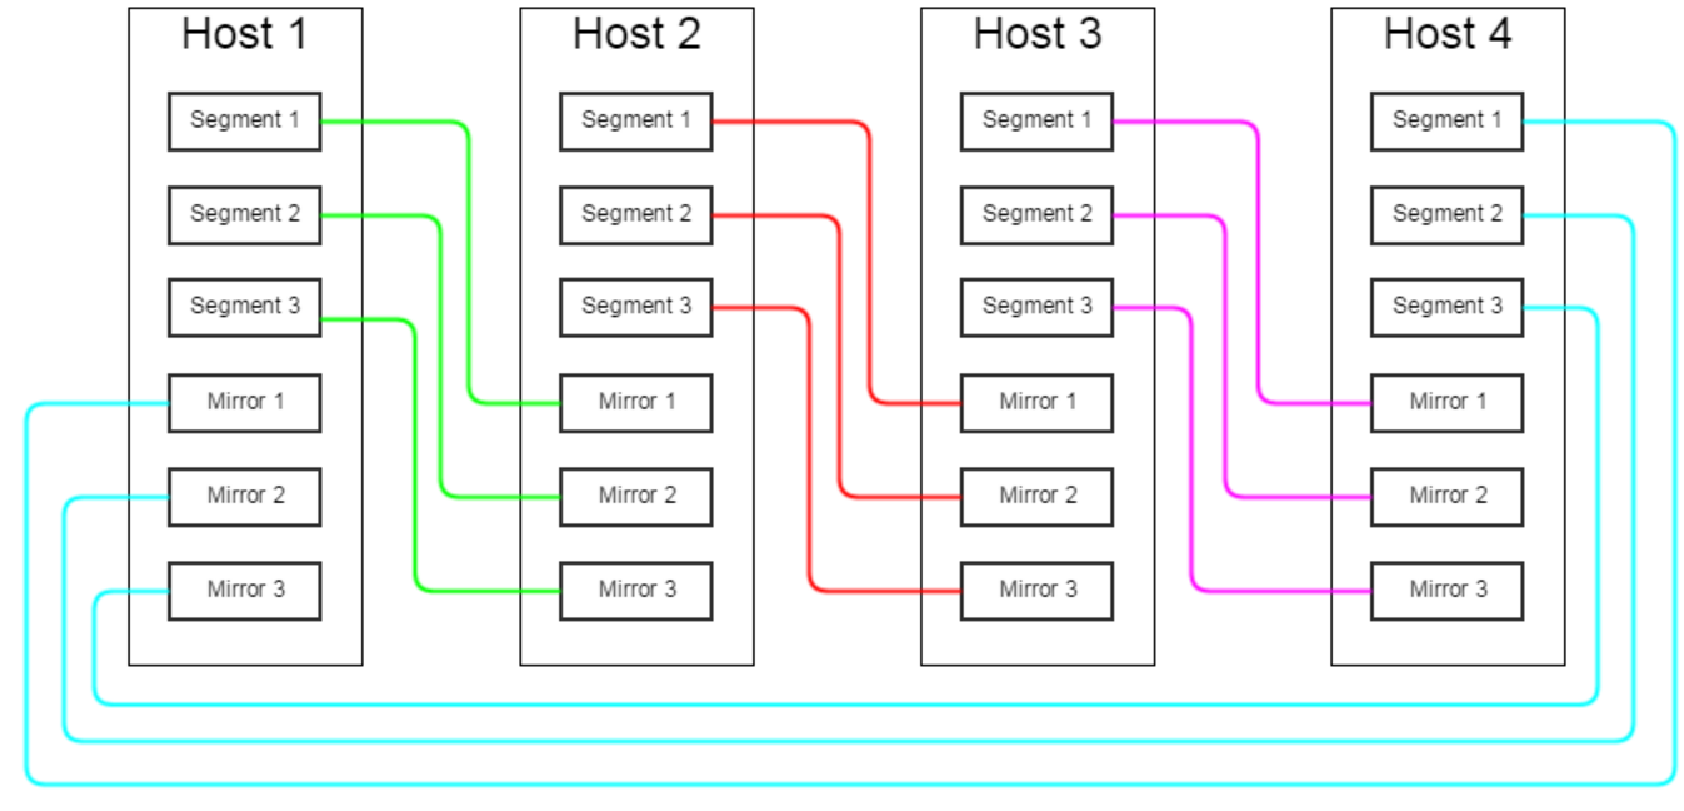
\includegraphics[width=1\textwidth]{greenplum-reserving-one.pdf}}
  \caption{Все зеркала сегментов, располагающихся на хосте N, находятся на хосте N+1}
  \label{fig:greenplum_reserve_one}
\end{figure}

При использовании схемы~\ref{fig:greenplum_reserve_one} при отказе одного из серверов на сервере-соседе оказывается в два раза больше работающих сегментов. Как было сказано выше, производительность кластера равняется производительности самого медленного из сегментов, а значит, в случае отказа одного сервера производительность базы снижается минимум вдвое. Однако, такая схема имеет и положительные стороны: при работе с отказавшим сервером уязвимым местом кластера становится только один сервер~--- тот самый, куда переехали сегменты.

\begin{figure}[ht!]
  \center{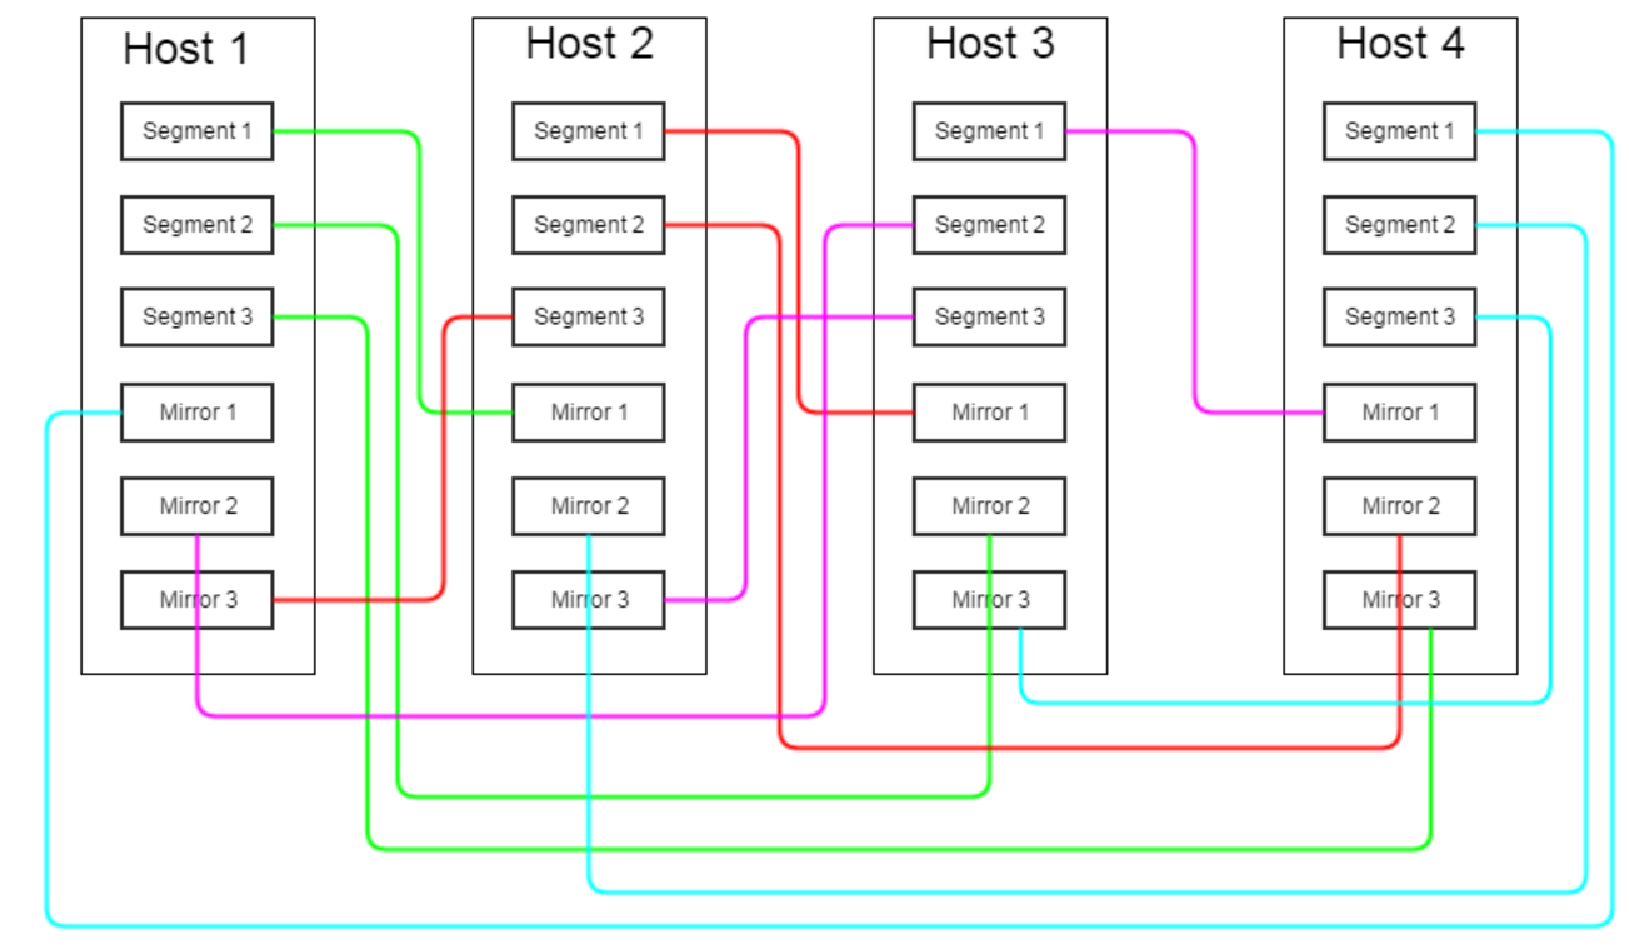
\includegraphics[width=1\textwidth]{greenplum-reserving-two.pdf}}
  \caption{Все зеркала сегментов, располагающихся на хосте N, равномерно <<мажутся>> на сервера N+1, N+2 ... N+M, где M – число сегментов на сервере}
  \label{fig:greenplum_reserve_two}
\end{figure}

При использовании схемы~\ref{fig:greenplum_reserve_two} в случае отказа сервера возросшая нагрузка равномерно распределяется между несколькими серверами, не сильно влияя на общую производительность кластера. Однако, существенно повышается риск выхода из строя всего кластера~--- достаточно выйти из строя одному из M серверов, соседствующих с вышедшим из строя изначально.

Истина, как это часто бывает, где-то посередине~--- можно расположить по несколько зеркал сегментов одного сервера на нескольких других серверах, можно объединять сервера в группы отказоустойчивости, и так далее. Оптимальную конфигурацию зеркал следует подбирать исходя из конкретных аппаратных данных кластера, критичности простоя и так далее.

Также в механизме резервирования сегментов есть ещё один нюанс, влияющий на производительность кластера. В случае выхода из строя зеркала одного из сегментов последний переходит в режим \lstinline!change tracking!~--- сегмент логирует все изменения, чтобы затем при восстановлении упавшего зеркала применить их к нему, и получить свежую, консистентную копию данных. Другими словами, при падении зеркала нагрузка, создаваемая на дисковую подсистему сервера сегментом, оставшимся без зеркала, существенно возрастает.

При устранении причины отказа сегмента (аппаратные проблемы, кончившееся место на устройстве хранения и прочее) его необходимо вернуть в работу вручную, с помощью специальной утилиты \lstinline!gprecoverseg! (даунтайм СУБД не требуется). По факту эта утилита скопирует скопившиеся на сегменте WA-логи на зеркало и поднимет упавший сегмент/зеркало. В случае, если речь идёт о primary-сегменте, изначально он включится в работу как зеркало для своего зеркала, ставшего primary (зеркало и основной сегмент будут работать поменявшись ролями). Для того, чтобы вернуть всё на круги своя, потребуется процедура ребаланса~--- смены ролей. Такая процедура также не требует даунтайма СУБД, однако на время ребаланса все сессии в БД подвиснут.

В случае, если повреждения упавшего сегмента настолько серьёзны, что простым копированием данных из WA-логов не обойтись, есть возможность использовать полное восстановление упавшего сегмента~--- в таком случае, по факту, инстанс PostgreSQL будет создан заново, однако за счёт того, что восстановление будет не инкрементальным, процесс восстановления может занять продолжительное время.


\subsection{Производительность}

Оценка производительности кластера Greenplum – понятие довольно растяжимое. Исходные данные: кластер из 24 сегмент-серверов, каждый сервер~--- 192 Гб памяти, 40 ядер. Число primary-сегментов в кластере: 96. В первом примере мы создаём таблицу с 4-я полями + первичный ключ по одному из полей. Затем мы наполняем таблицу данными (10 000 000 строк) и пробуем выполнить простой \lstinline!SELECT! с несколькими условиями.

\begin{lstlisting}[language=SQL,label=lst:greenplum_example5,caption=SELECT с условиями]
db=# CREATE TABLE test3
db-# (id bigint NOT NULL,
db(# profile bigint NOT NULL,
db(# status integer NOT NULL,
db(# switch_date timestamp without time zone NOT NULL,
db(# CONSTRAINT test3_id_pkey PRIMARY KEY (id) )
db-# distributed by (id);
NOTICE:  CREATE TABLE / PRIMARY KEY will create implicit index "test3_pkey" for table "test3"
CREATE TABLE

db=# insert into test3 (id , profile,status, switch_date) select a, round(random()*100000), round(random()*4), now() - '1 year'::interval * round(random() * 40) from generate_series(1,10000000) a;
INSERT 0 10000000

db=# explain analyze  select  profile, count(status) from test3
db=#                         where status<>2
db=#                         and switch_date between '1970-01-01' and '2015-01-01'  group by profile;

Gather Motion 96:1 (slice2; segments: 96) (cost=2092.80..2092.93 rows=10 width=16)
Rows out: 100001 rows at destination with 141 ms to first row, 169 ms to end, start offset by 0.778 ms.
-> HashAggregate (cost=2092.80..2092.93 rows=1 width=16)
   Group By: test3.profile
   Rows out: Avg 1041.7 rows x 96 workers. Max 1061 rows (seg20) with 141 ms to end, start offset by 2.281 ms.
   Executor memory: 4233K bytes avg, 4233K bytes max (seg0).
   -> Redistribute Motion 96:96 (slice1; segments: 96) (cost=2092.45..2092.65 rows=1 width=16)
      Hash Key: test3.profile
      Rows out: Avg 53770.2 rows x 96 workers at destination. Max 54896 rows (seg20) with 71 ms to first row, 117 ms to end, start offset by 5.205 ms.
      -> HashAggregate (cost=2092.45..2092.45 rows=1 width=16)
      Group By: test3.profile
      Rows out: Avg 53770.2 rows x 96 workers. Max 54020 rows (seg69) with 71 ms to first row, 90 ms to end, start offset by 7.014 ms.
      Executor memory: 7882K bytes avg, 7882K bytes max (seg0).
      -> Seq Scan on test3 (cost=0.00..2087.04 rows=12 width=12)
         Filter: status <> 2 AND switch_date >= '1970-01-01 00:00:00'::timestamp without time zone AND switch_date <= '2015-01-01 00:00:00'::timestamp without time zone
         Rows out: Avg 77155.1 rows x 96 workers. Max 77743 rows (seg26) with 0.092 ms to first row, 31 ms to end, start offset by 7.881 ms.
Slice statistics:
(slice0) Executor memory: 364K bytes.
(slice1) Executor memory: 9675K bytes avg x 96 workers, 9675K bytes max (seg0).
(slice2) Executor memory: 4526K bytes avg x 96 workers, 4526K bytes max (seg0).
Statement statistics:
Memory used: 128000K bytes
Total runtime: 175.859 ms
\end{lstlisting}

Как видно, время выполнения запроса составило 175 мс. Теперь попробуем пример с джойном по ключу дистрибуции одной таблицы и по обычному полю другой таблицы.

\begin{lstlisting}[language=SQL,label=lst:greenplum_example6,caption=JOIN по ключу дистрибуции одной таблицы и по обычному полю другой]
db=# create table test3_1 (id bigint NOT NULL, name text, CONSTRAINT test3_1_id_pkey PRIMARY KEY (id)) distributed by (id);
NOTICE:  CREATE TABLE / PRIMARY KEY will create implicit index "test3_1_pkey" for table "test3_1"
CREATE TABLE
db=# insert into test3_1 (id , name) select a, md5(random()::text) from generate_series(1,100000) a;
INSERT 0 100000
db=# explain analyze select test3.*,test3_1.name from test3 join test3_1 on test3.profile=test3_1.id;

-> Hash Join (cost=34.52..5099.48 rows=1128 width=60)
   Hash Cond: test3.profile = test3_1.id
   Rows out: Avg 104166.2 rows x 96 workers. Max 106093 rows (seg20) with 7.644 ms to first row, 103 ms to end, start offset by 223 ms.
   Executor memory: 74K bytes avg, 75K bytes max (seg20).
   Work_mem used: 74K bytes avg, 75K bytes max (seg20). Workfile: (0 spilling, 0 reused)
   (seg20) Hash chain length 1.0 avg, 1 max, using 1061 of 262151 buckets.
   -> Redistribute Motion 96:96 (slice1; segments: 96) (cost=0.00..3440.64 rows=1128 width=28)
      Hash Key: test3.profile
      Rows out: Avg 104166.7 rows x 96 workers at destination. Max 106093 rows (seg20) with 3.160 ms to first row, 44 ms to end, start offset by 228 ms.
      -> Seq Scan on test3 (cost=0.00..1274.88 rows=1128 width=28)
      Rows out: Avg 104166.7 rows x 96 workers. Max 104209 rows (seg66) with 0.165 ms to first row, 16 ms to end, start offset by 228 ms.
   -> Hash (cost=17.01..17.01 rows=15 width=40)
      Rows in: Avg 1041.7 rows x 96 workers. Max 1061 rows (seg20) with 1.059 ms to end, start offset by 227 ms.
      -> Seq Scan on test3_1 (cost=0.00..17.01 rows=15 width=40)
         Rows out: Avg 1041.7 rows x 96 workers. Max 1061 rows (seg20) with 0.126 ms to first row, 0.498 ms to end, start offset by 227 ms.
Slice statistics:
(slice0) Executor memory: 364K bytes.
(slice1) Executor memory: 1805K bytes avg x 96 workers, 1805K bytes max (seg0).
(slice2) Executor memory: 4710K bytes avg x 96 workers, 4710K bytes max (seg0). Work_mem: 75K bytes max.
Statement statistics:
Memory used: 128000K bytes
Total runtime: 4526.065 ms
\end{lstlisting}

Время выполнения запроса составило 4.6 секунды. Много это или мало для такого объёма данных~--- вопрос спорный и лежащий вне этой книги.



\subsection{Расширение кластера}

В жизненном цикле распределённой аналитической БД рано или поздно возникает ситуация, когда объём доступного дискового пространства уже не может вместить всех необходимых данных, а добавление устройств хранения в имеющиеся сервера либо невозможна, либо слишком дорога и сложна (потребуется, как минимум, расширение существующих разделов). Кроме того, добавление одних лишь дисковых мощностей негативно скажется на соотношении <<число процессоров/Тб данных>>, о котором мы говорили в <<\ref{subsec:greenplum_data_storage}~\nameref{subsec:greenplum_data_storage}>>. Говоря простым языком, в кластер рано или поздно понадобится вводить новые сервера. Greenplum позволяет добавлять как новые сервера, так и новые сегменты практически без простоя СУБД. Последовательность этого действа примерно такая:

\begin{itemize}
  \item разработать карту сегментов, согласно которой GP будет размещать новые сегменты и зеркала на новых серверах;
  \item сделать бекап необходимых критичных данных (как минимум всех метаданных);
  \item установить ПО СУБД на новые сервера;
  \item остановить СУБД (следующий пункт выполняется в даунтайм);
  \item инициализировать новые сегменты утилитой \lstinline!gpexpand! (занимает от 5 до 10 минут);
  \item поднять СУБД (даунтайм окончен);
  \item перераспределить (redistribute) все таблицы;
  \item собрать статистику (analyze) по всем таблицам;
\end{itemize}

Как видно, хотя процедура расширения и продолжительна, полная недоступность БД при правильных действиях администратора не превысит 20-30 минут.


\subsection{Особенности эксплуатации}

Как обычно, практика вносит в красивую теорию свои коррективы. Поделюсь некоторыми нюансами эксплуатации, выявленными нами за долгое время использования GP. Сразу оговорюсь, что стандартные нюансы PostgreSQL (необходимость \lstinline!VACUUM!, особенности репликации) в этот перечень не попали:

\begin{itemize}
  \item Автоматический failover не даёт 100\% гарантии переключения на зеркало. Увы, но это так, особенно под нагрузкой, есть риск зависания процессов базы при попытке переключения на зеркало. Частично проблему решает уменьшение таймаута ответа от сегментов до нескольких минут, однако даже в таком случае риск остаётся. Как частное решение проблемы зависания при переключении можно использовать ручное убийство зависшего сегмента или перезагрузку базы;
  \item Greenplum и OLTP несовместимы. GP~--- аналитическая БД, предназначенная для небольшого числа одновременных запросов, выполняющих тяжёлые операции над большим объёмом данных. Большое число (более 600 queries per second) лёгких запросов/транзакций, выполняющих одну операцию, негативно сказывается на производительности базы из-за её распределённой архитектуры~--- каждая транзакция на мастере порождает N транзакций на сегментах. Хорошей практикой является агрегация большого числа \lstinline!UPDATE/INSERT! в батчи;
  \item Отсутствие механизма инкрементального бекапа;
  \item Свой синтаксис. Несмотря на то, что для клиента Greenplum по сути является PostgreSQL DB, небольшие различия в синтаксисе SQL заставляют использовать стандартный клиентский PostgreSQL-софт с большой осторожностью;
  \item Отсутствие возможности пометить сегменты как <<архивные>>. Частично этот недостаток можно решить путём использования архивных партиций, находящихся на медленном дешевом tablespace, а также c помощью появившейся в последней на момент написания главы версии GP 4.3.6.0 возможности располагать партиции таблицы во внешних источниках (например, внешних таблицах \lstinline!gphdfs!, лежащих в кластере Hadoop);
  \item Greenplum использует PostgreSQL версии 8.3.23, а значит о многих современных плюшках этой замечательной БД придётся забыть;
\end{itemize}


\subsection{Заключение}

Greenplum~--- мощный и гибкий инструмент для аналитической обработки больших объёмов данных. Он требует к себе немного другого подхода, чем остальные enterprise-level решения для Data Warehouse (<<напильник>>~--- любимый инструмент администратора GP). Однако при достаточно низком пороге вхождения и большой унифицированности с PostgreSQL Greenplum является сильным игроком на поле Data Warehouse DB.
